\documentclass[10pt]{article}

\usepackage[a4paper, left=2cm, right=2cm]{geometry} % A4 paper size and thin margins

\usepackage{graphicx}
\graphicspath{ {../imgs/} }

\usepackage{blindtext}
\usepackage{everypage}
\usepackage{environ}
\newcounter{abspage}

\usepackage{hyperref}

\usepackage{xcolor}

\usepackage[utf8]{inputenc}
\usepackage[T1]{fontenc}
\usepackage[sfdefault]{ClearSans}

\makeatletter
\newcommand{\newSFPage}[1]
  {\global\expandafter\let\csname SFPage@#1\endcsname\null}

\NewEnviron{SidewaysFigure}{\begin{figure}[p]
\protected@write\@auxout{\let\theabspage=\relax}% delays expansion until shipout
  {\string\newSFPage{\theabspage}}%
\ifdim\textwidth=\textheight
  \rotatebox{90}{\parbox[c][\textwidth][c]{\linewidth}{\BODY}}%
\else
  \rotatebox{90}{\parbox[c][\textwidth][c]{\textheight}{\BODY}}%
\fi
\end{figure}}

\AddEverypageHook{% check if sideways figure on this page
  \ifdim\textwidth=\textheight
    \stepcounter{abspage}% already in landscape
  \else
    \@ifundefined{SFPage@\theabspage}{}{\global\pdfpageattr{/Rotate 0}}%
    \stepcounter{abspage}%
    \@ifundefined{SFPage@\theabspage}{}{\global\pdfpageattr{/Rotate 90}}%
  \fi}
\makeatother


\begin{document}


\begin{titlepage}
		\parbox[t]{0.93\textwidth}{
			\parbox[t]{0.91\textwidth}{
				\raggedright
				\fontsize{50pt}{80pt}\selectfont
				\vspace{0.7cm}
				
\includegraphics[width=0.5\textwidth]{DPI_logo.png}
				
				Clyde River Water\\
				Quality Report\\
				\vspace{0.7cm}
			}
		}
	\vfill
	\parbox[t]{0.93\textwidth}{ 
		\raggedleft
		\large
		{\Large Climate Smart Pilots}\\[4pt] 
		\today \\
		\vspace{0.5cm}
		\texttt{www.farmdecisiontech.net.au}\\
		
		\hfill\rule{0.2\linewidth}{1pt}
	}
\end{titlepage}

\section*{Foreword}

\subsection*{Funding}
This work has been produced by the NSW Primary Industries Climate Change Research Strategy funded by the NSW Climate Change Fund.

\subsection*{NSW Department of Primary Industries Disclaimer}
This is a research trial and pilot project, and you should not rely solely on the information or advice provided in these reports.

\subsection*{NSW Food Authority Disclaimer}
The NSW Food Authority attempts to ensure this information is updated regularly. Due to the unpredictable nature of events leading to harvesting closures, and the fact they may not always occur during business hours, the list may not always reflect the most recent closures and conditions and is not intended to be legally binding. Before harvesting shellfish for human consumption, farmers should confirm the status of the Harvest Area.

\subsection*{Feedback and Questions}
Please provide feedback and questions to Harvey Bates \\ \\
Email: \href{mailto:harvey.bates@dpi.nsw.gov.au}{harvey.bates@dpi.nsw.gov.au} \\ \\
Ph: 0447 359 557


\begin{SidewaysFigure}
\centering
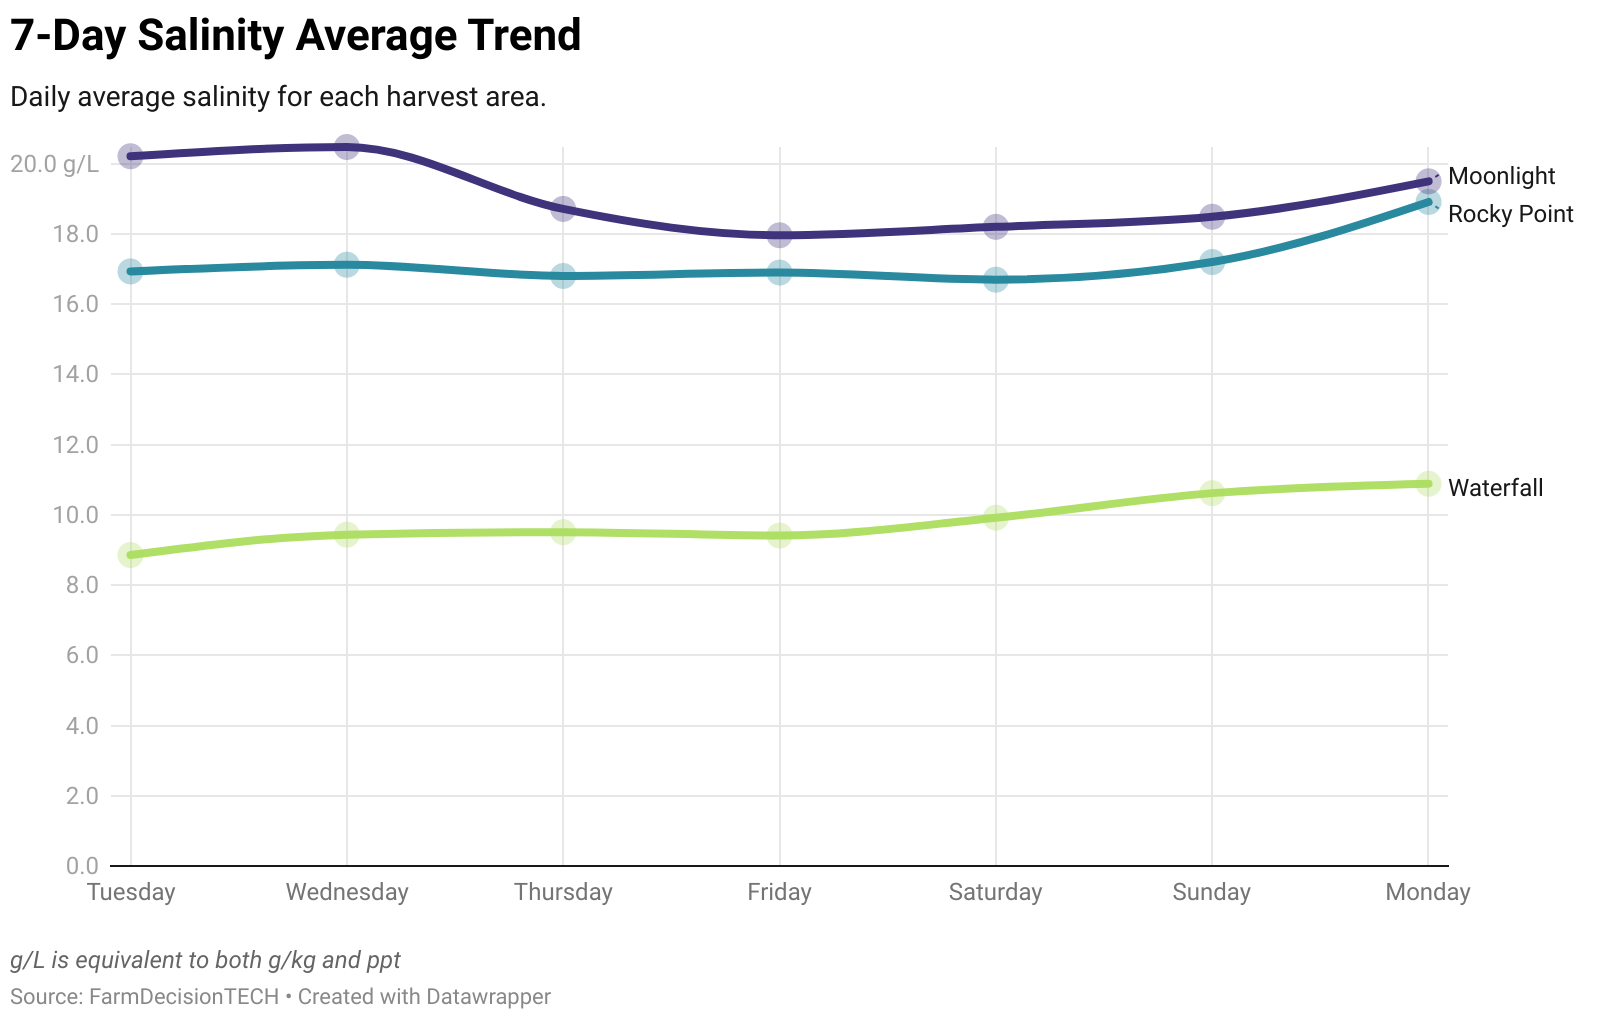
\includegraphics[width=1.3\textwidth]{weekly-salinity-chart.png}
\end{SidewaysFigure}
\vfill
\newpage

\begin{SidewaysFigure}
\centering
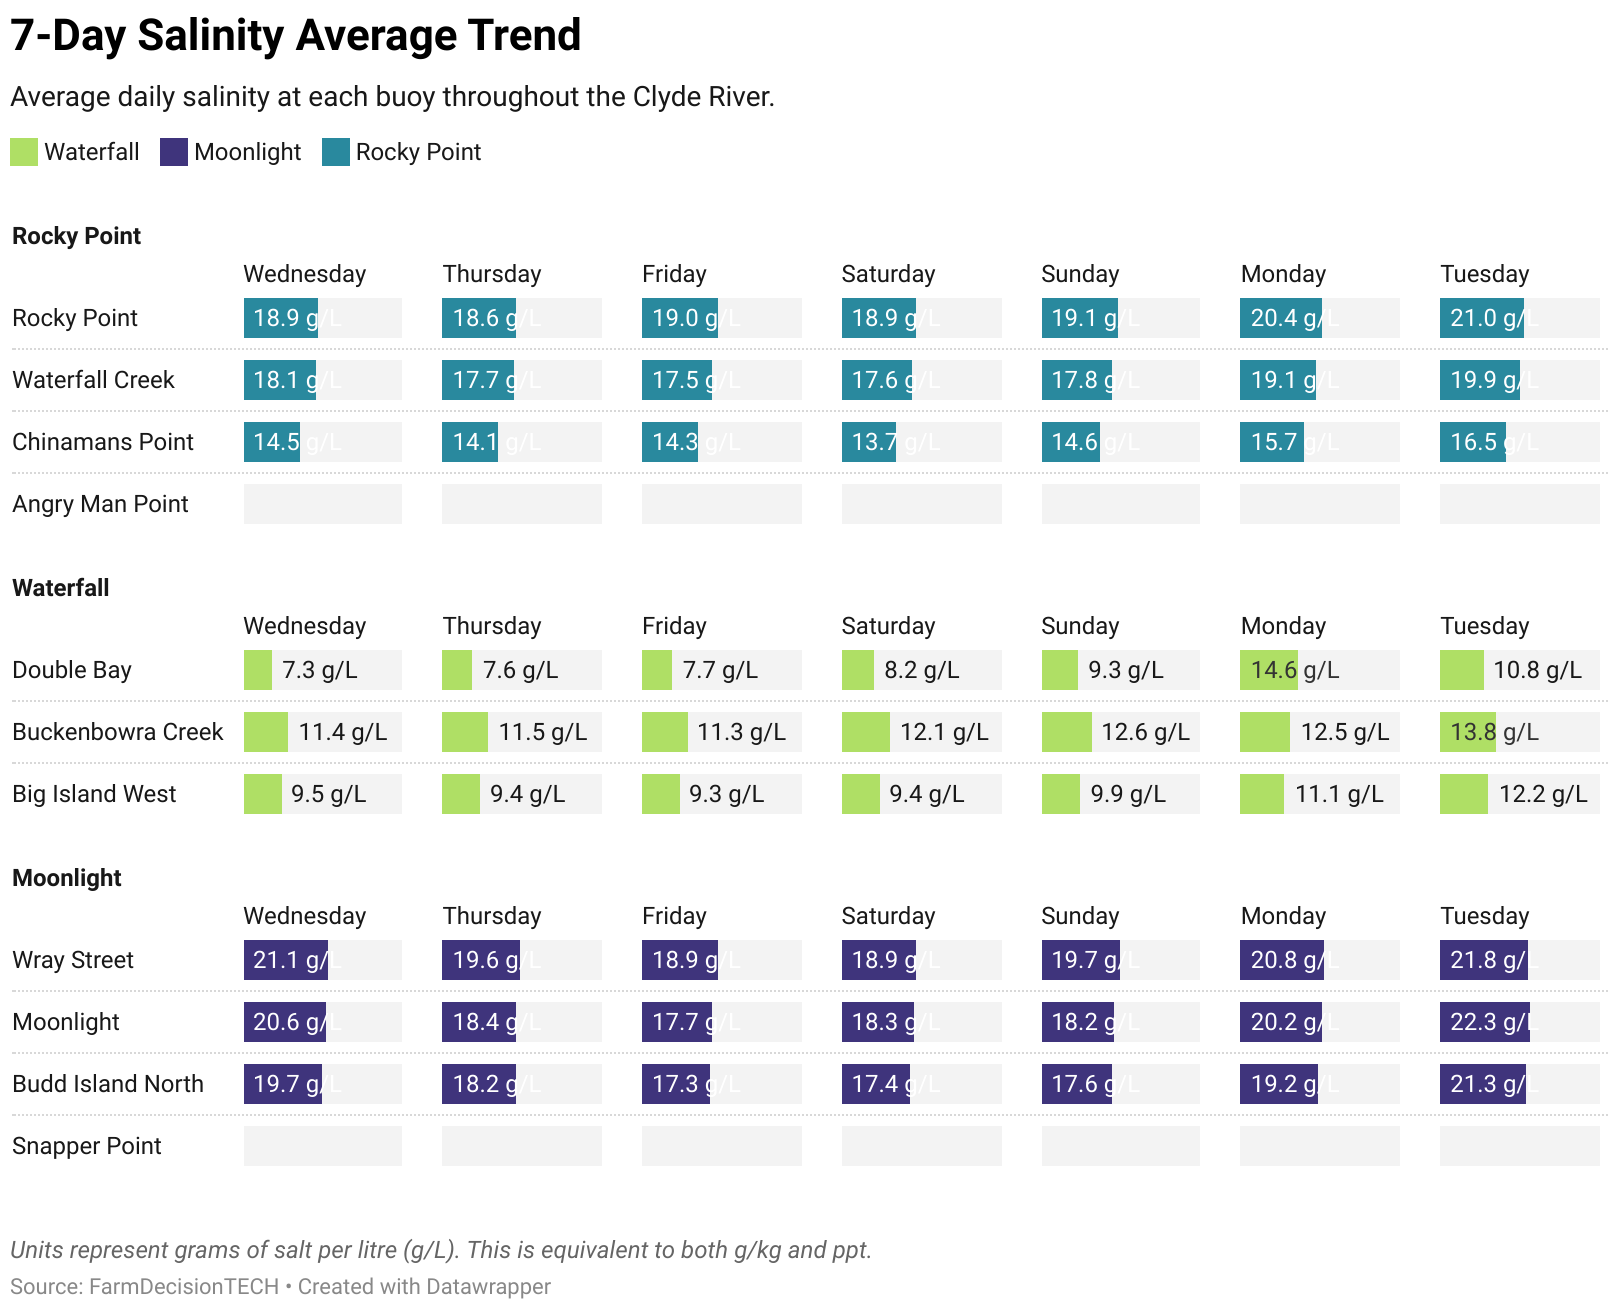
\includegraphics[width=1.3\textwidth]{weekly-salinity.png}
\end{SidewaysFigure}
\vfill
\newpage

\begin{SidewaysFigure}
\centering
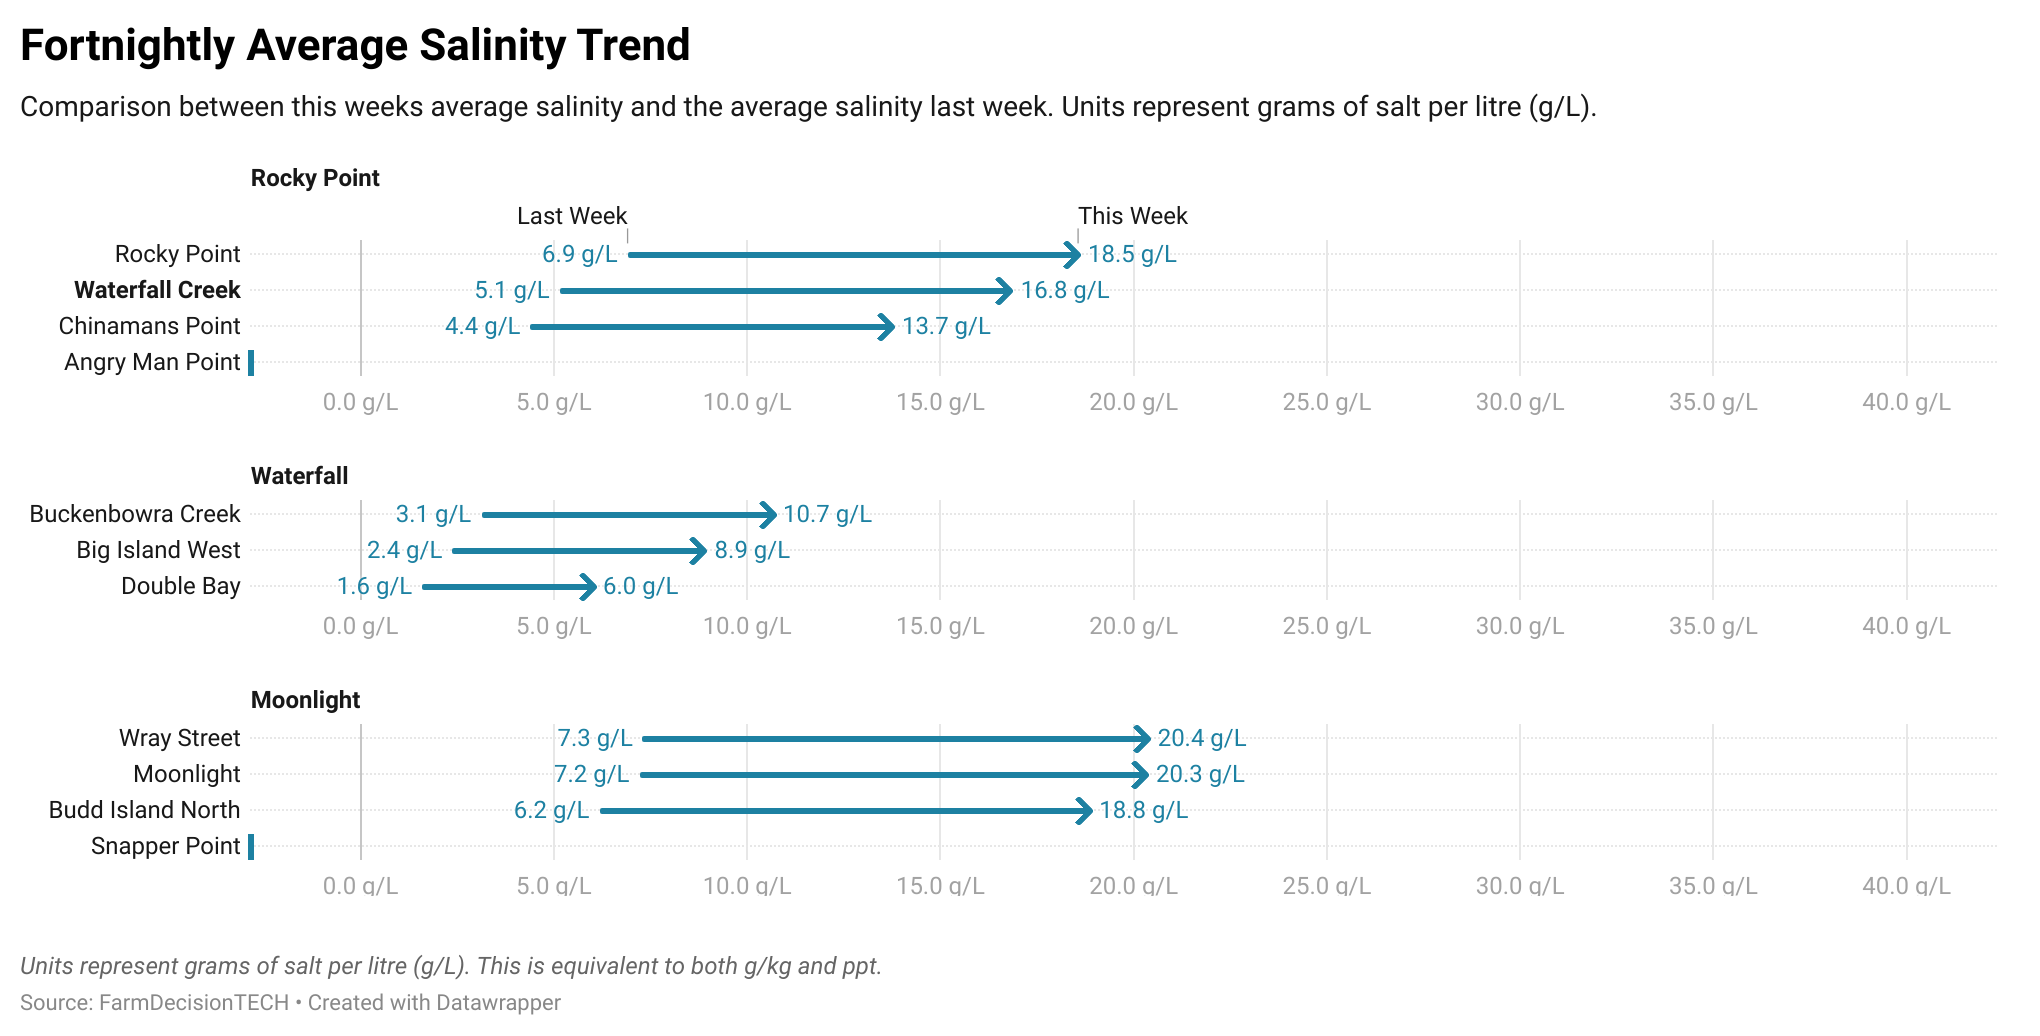
\includegraphics[width=1.3\textwidth]{fortnightly-salinity.png}
\end{SidewaysFigure}
\vfill
\newpage

\begin{SidewaysFigure}
\centering
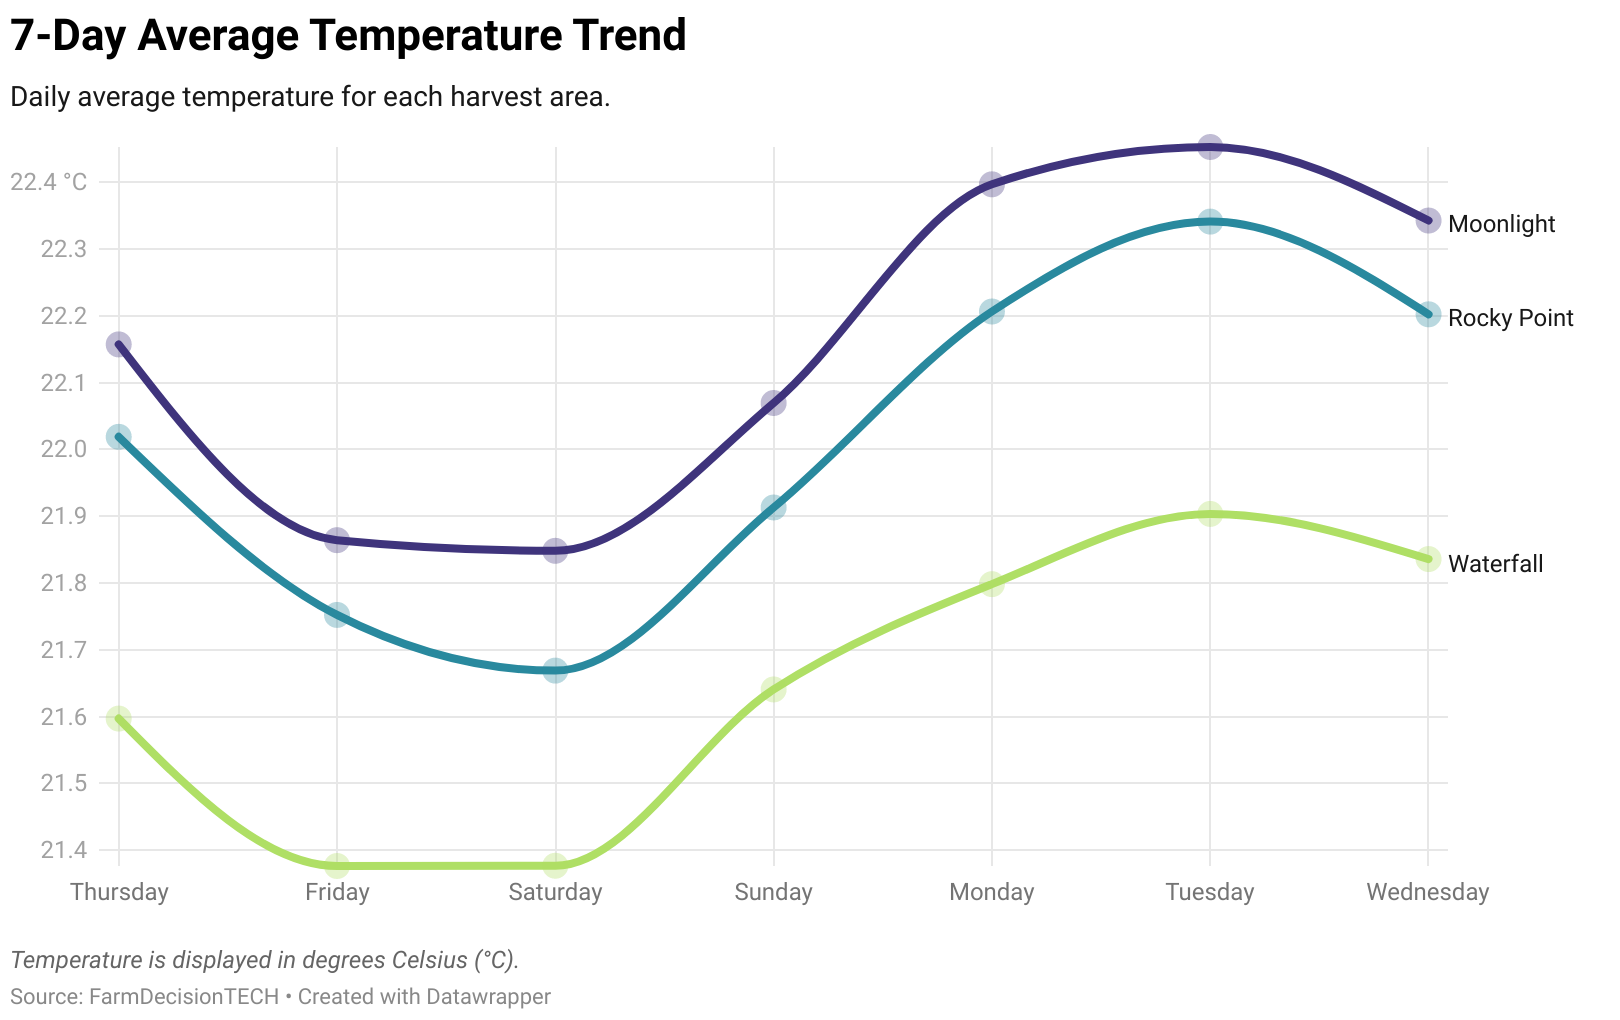
\includegraphics[width=1.3\textwidth]{weekly-temperature-chart.png}
\end{SidewaysFigure}
\vfill
\newpage

\begin{SidewaysFigure}
\centering
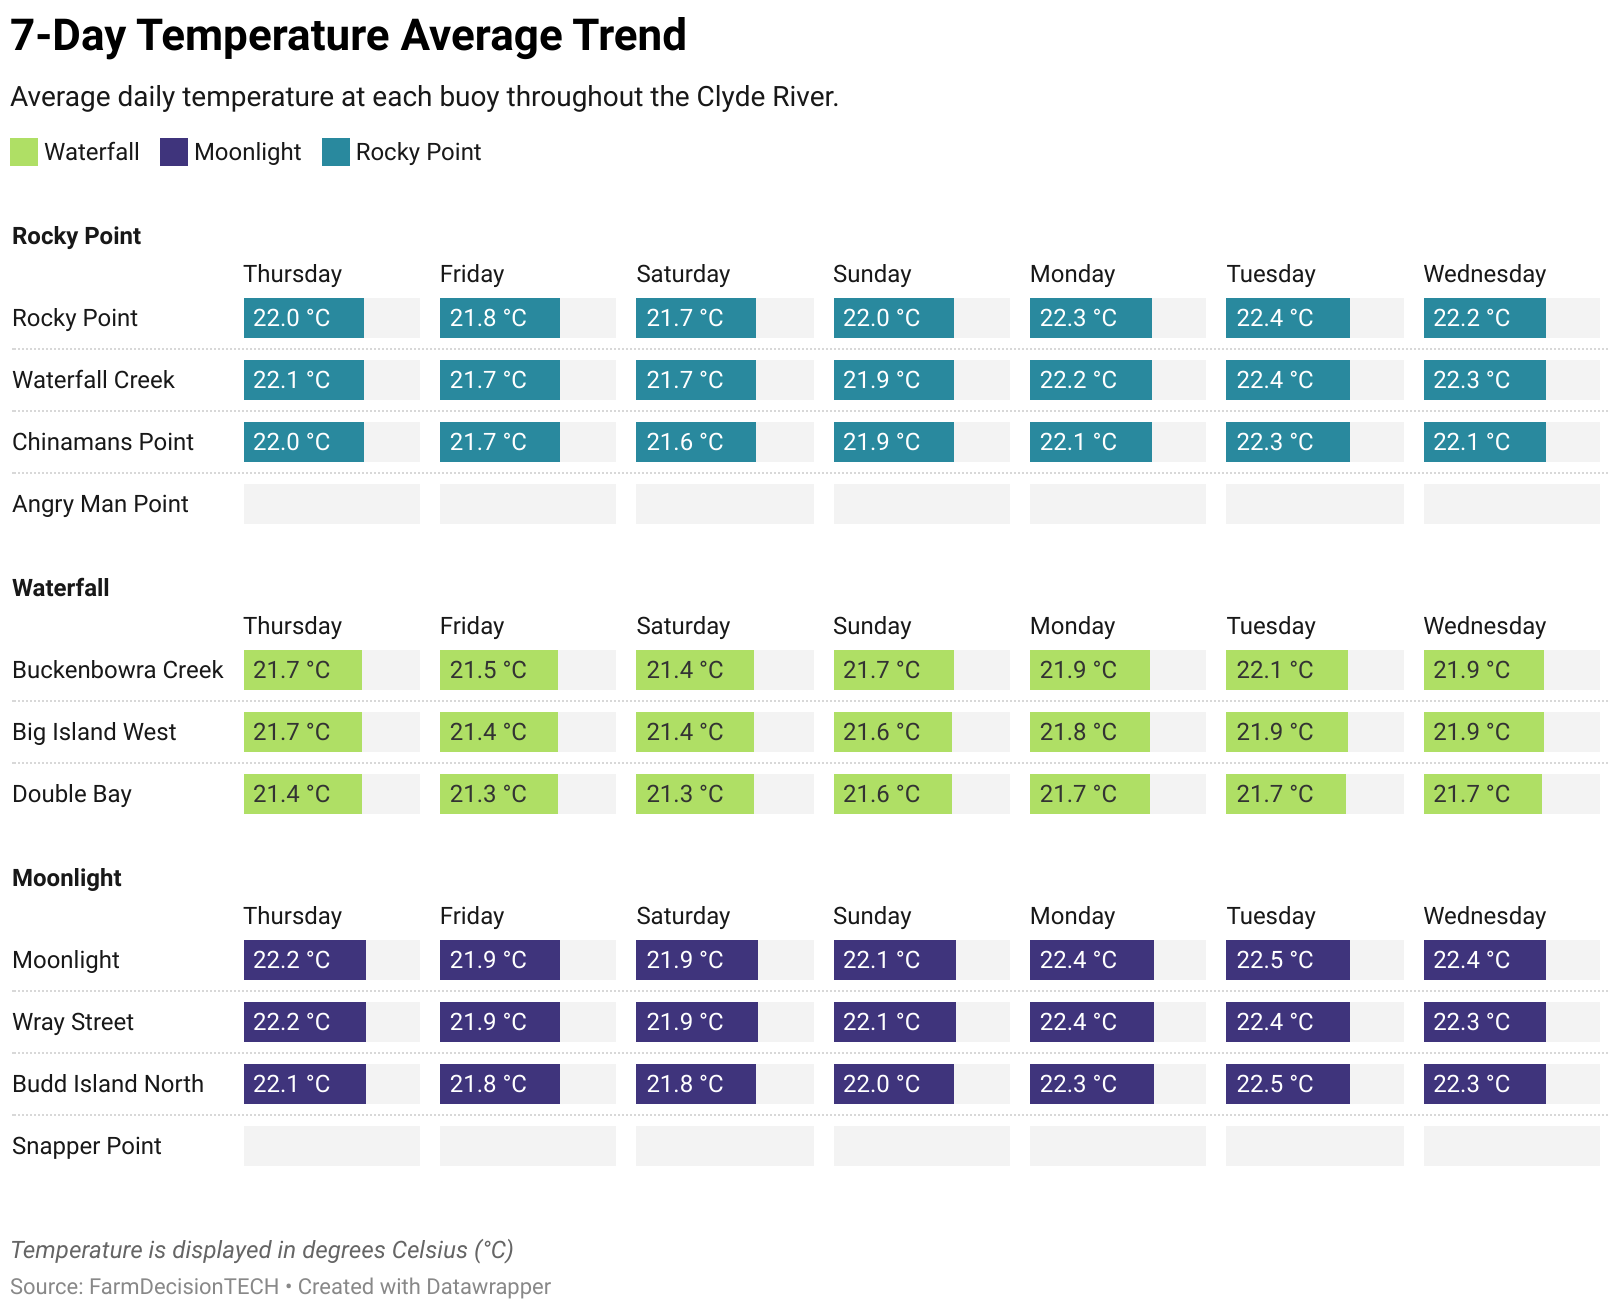
\includegraphics[width=1.3\textwidth]{weekly-temperature.png}
\end{SidewaysFigure}
\vfill
\newpage

\begin{SidewaysFigure}
\centering
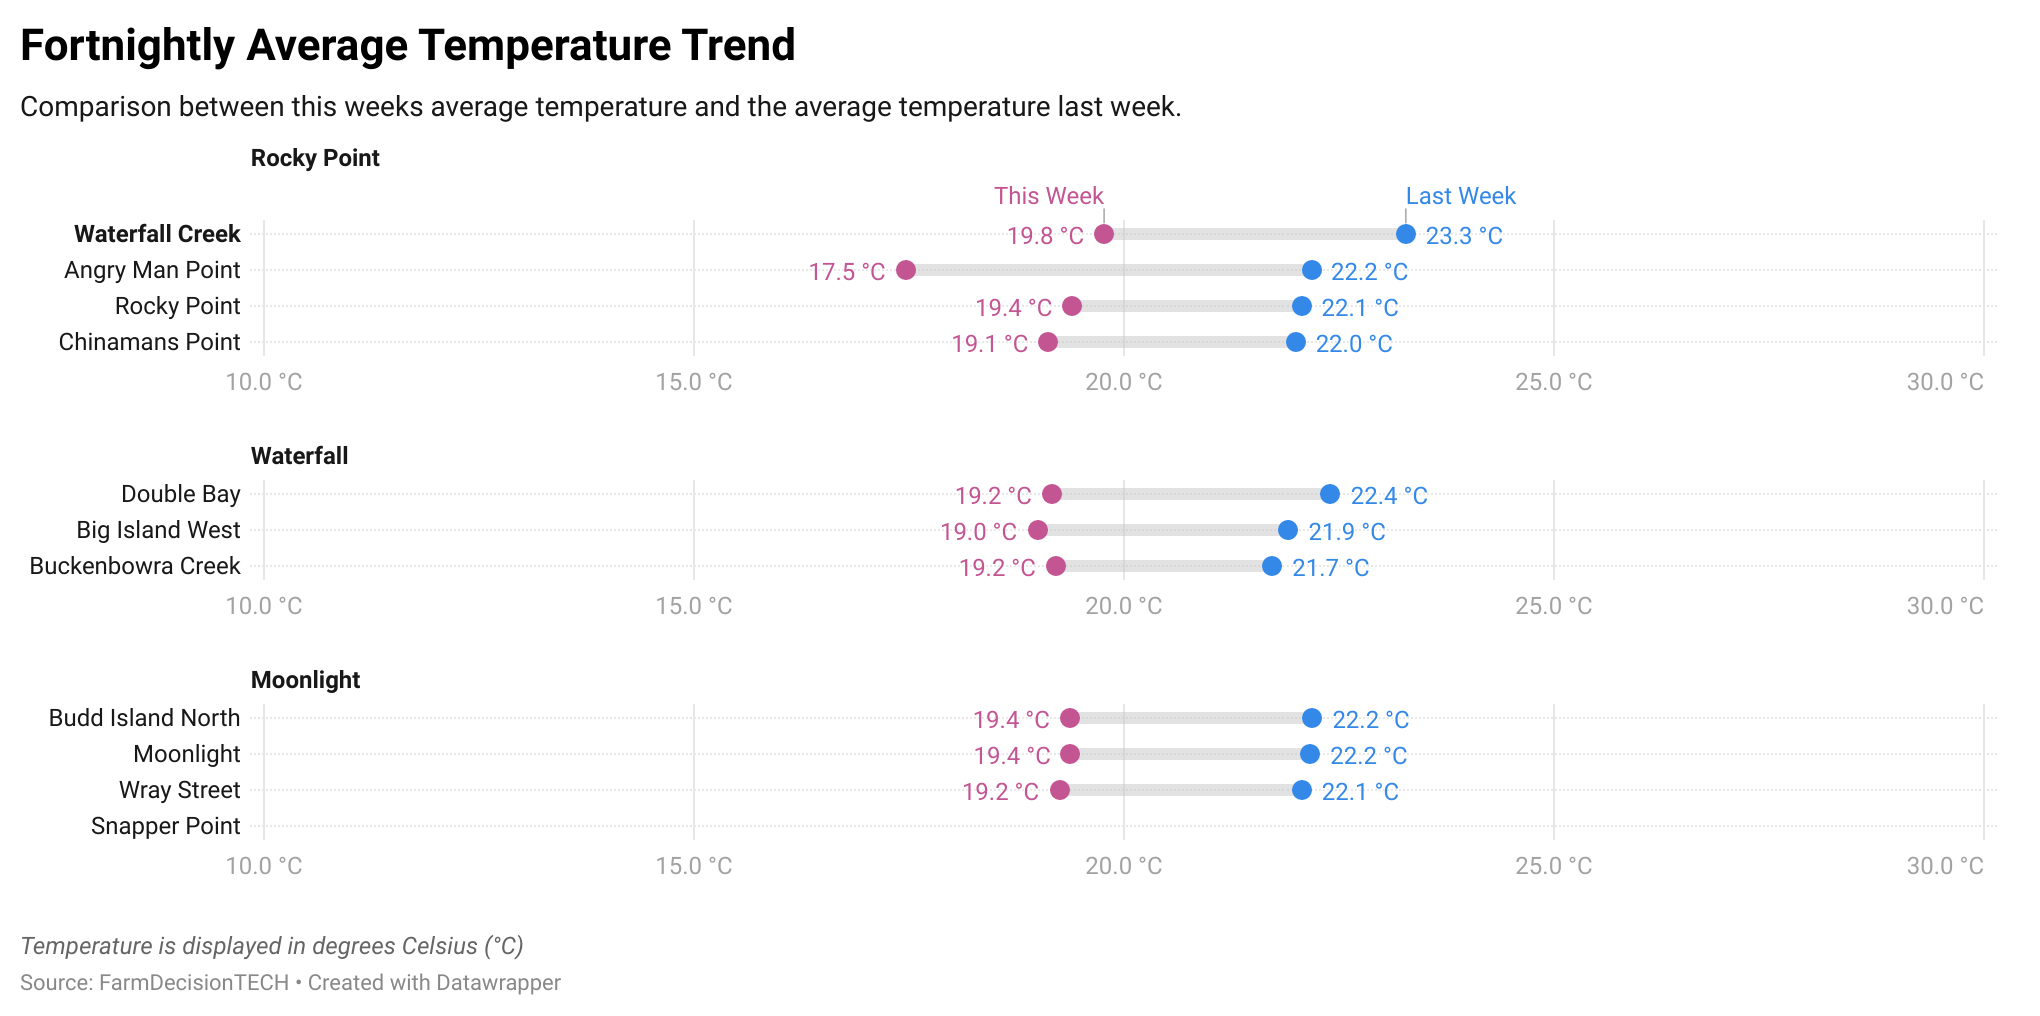
\includegraphics[width=1.3\textwidth]{fortnightly-temperature.png}
\end{SidewaysFigure}
\vfill
\newpage

\begin{SidewaysFigure}
\centering
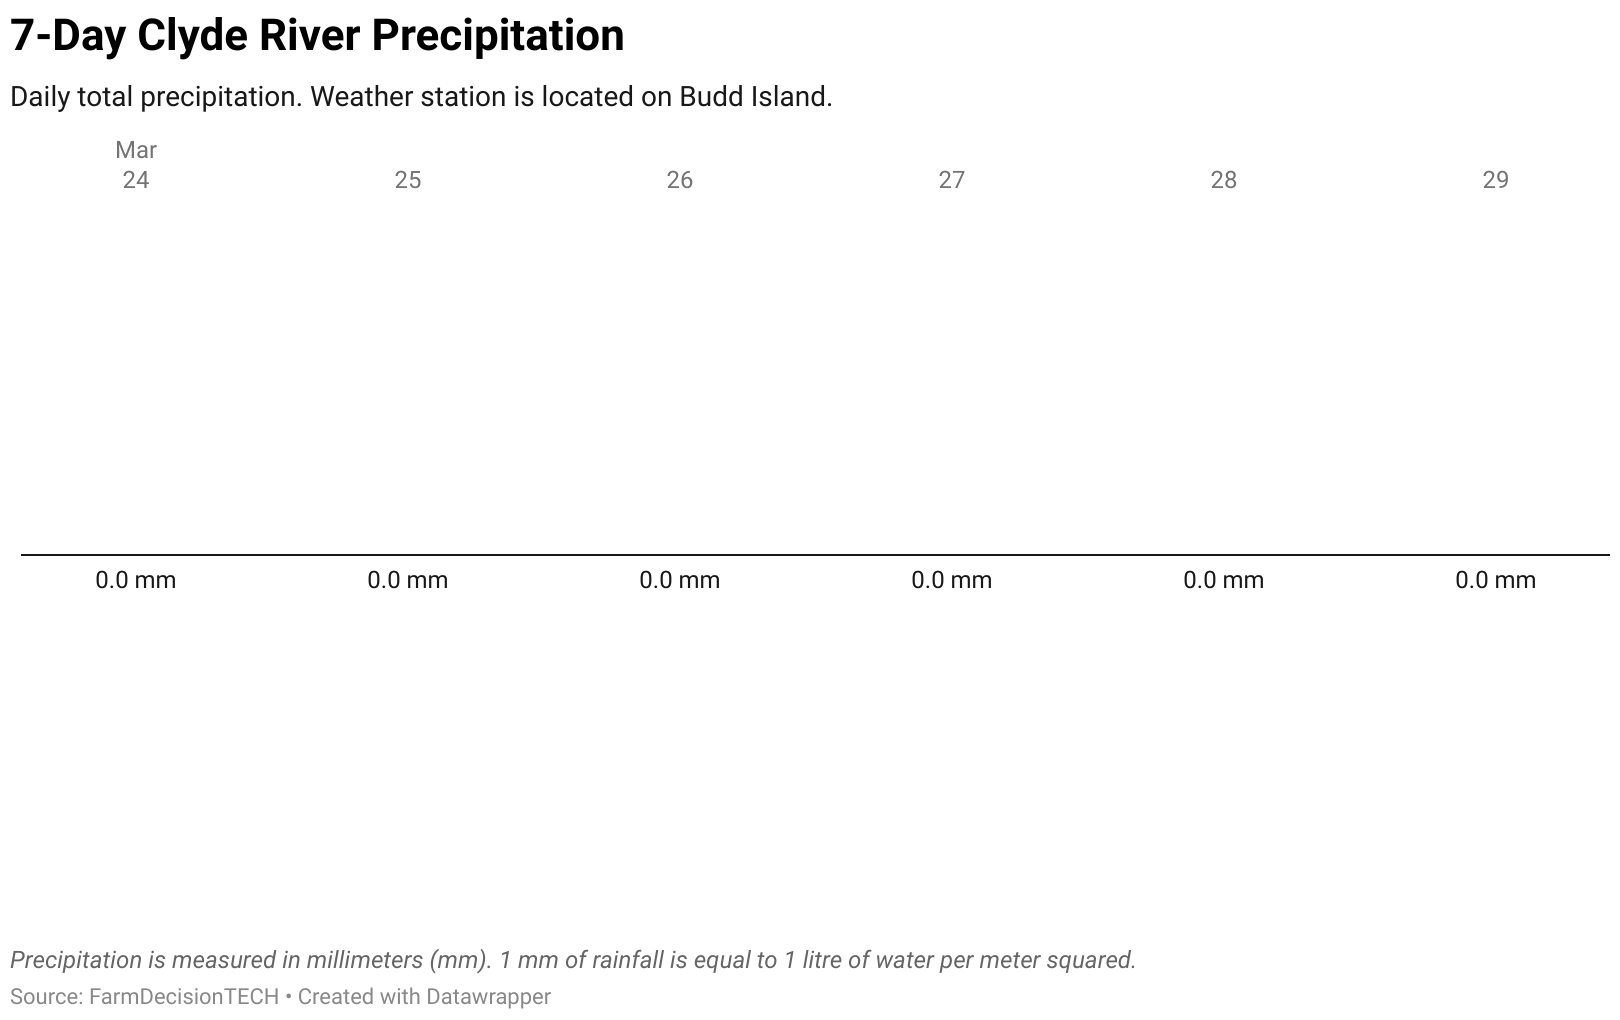
\includegraphics[width=1.3\textwidth]{weekly-precipitation.png}
\end{SidewaysFigure}
\vfill
\newpage

\begin{SidewaysFigure}
\centering
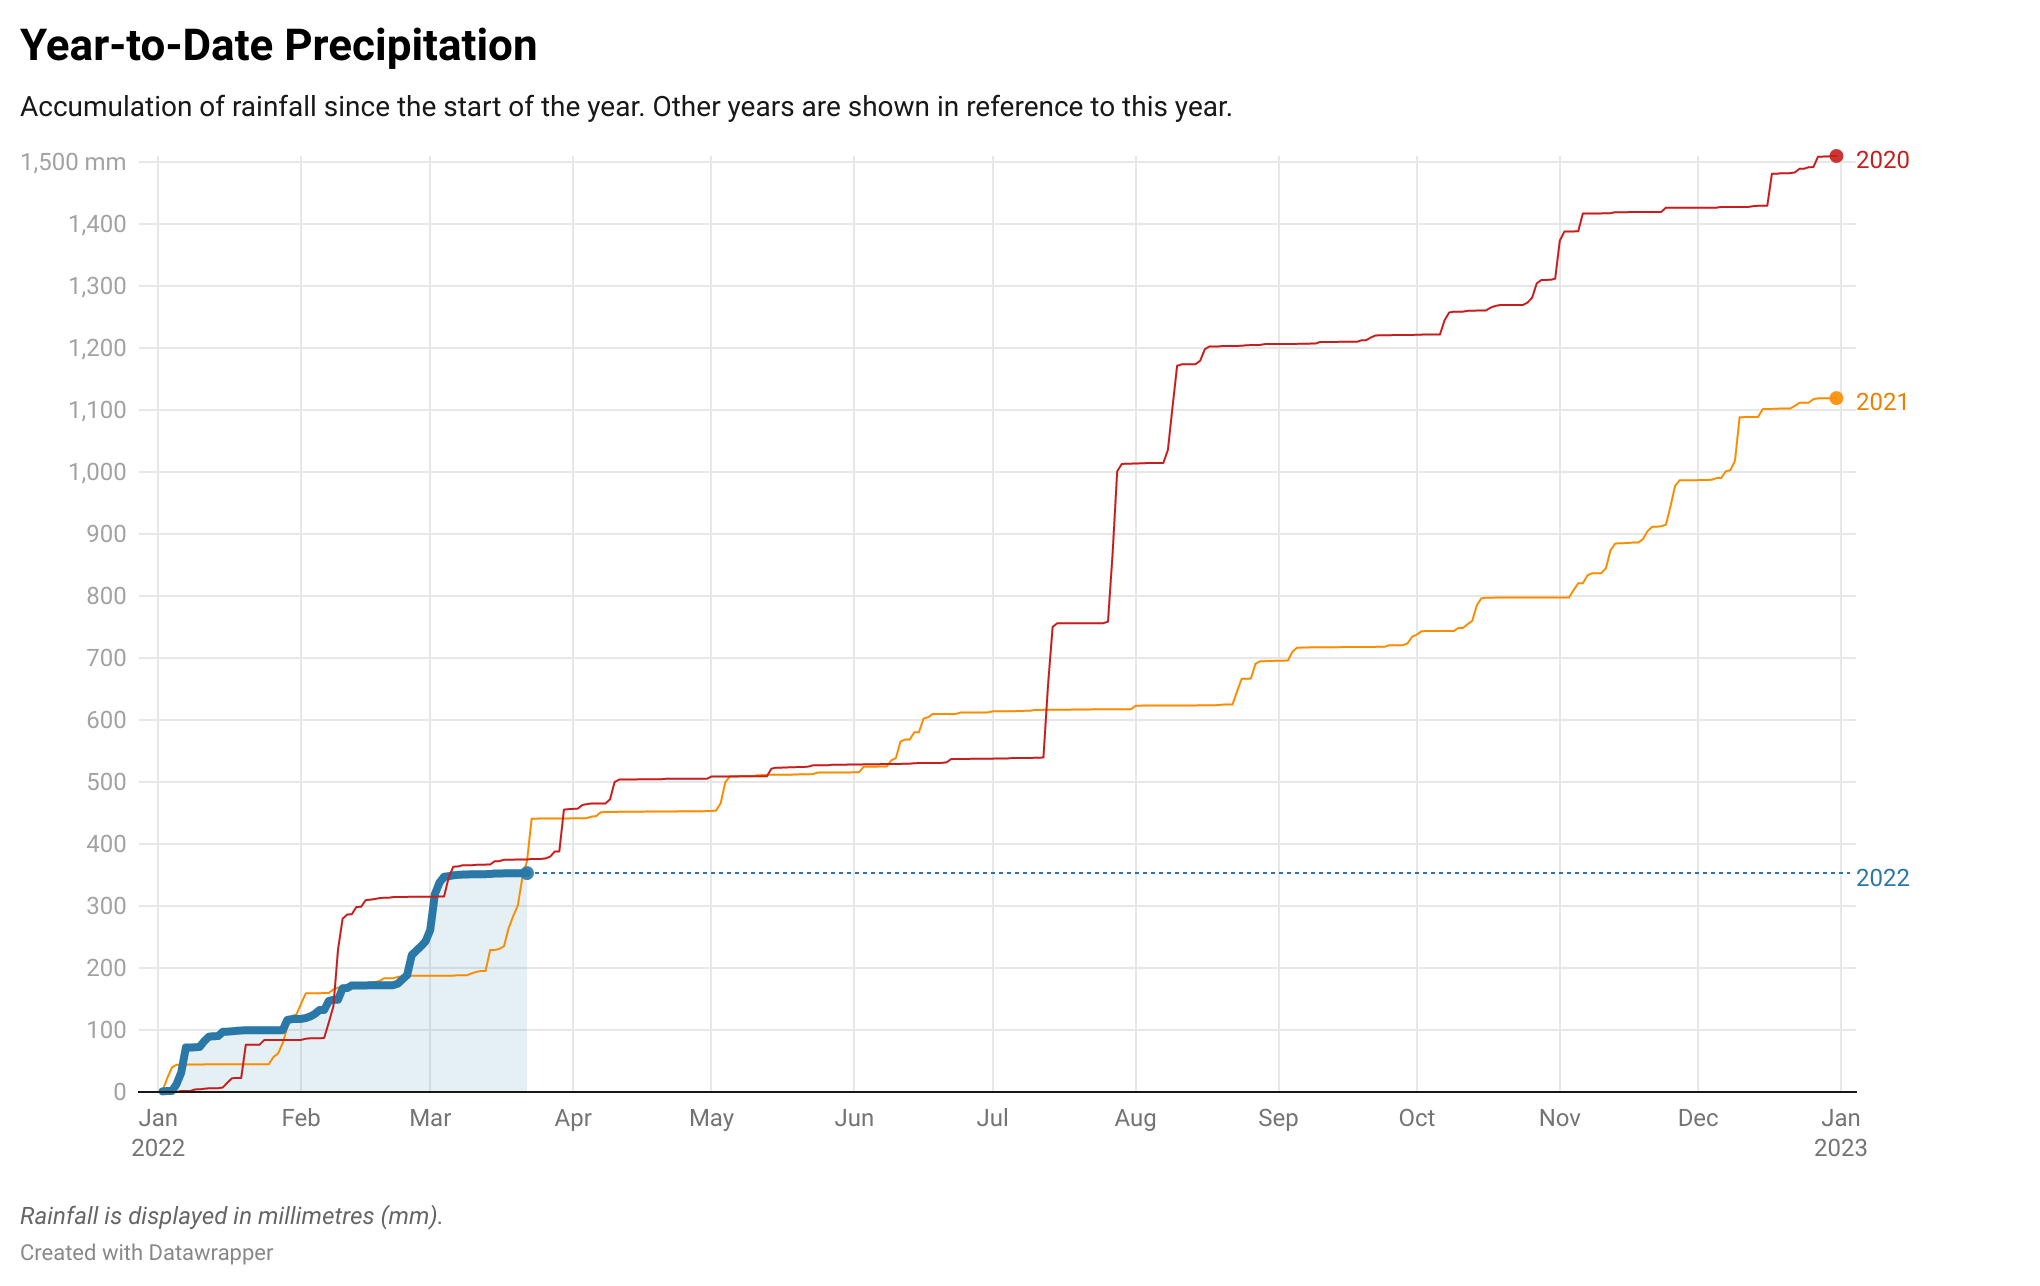
\includegraphics[width=1.3\textwidth]{yearly-precipitation.png}
\end{SidewaysFigure}
\vfill
\newpage

\end{document}